% This is "sig-alternate.tex" V2.0 May 2012
% This file should be compiled with V2.5 of "sig-alternate.cls" May 2012
%
% This example file demonstrates the use of the 'sig-alternate.cls'
% V2.5 LaTeX2e document class file. It is for those submitting
% articles to ACM Conference Proceedings WHO DO NOT WISH TO
% STRICTLY ADHERE TO THE SIGS (PUBS-BOARD-ENDORSED) STYLE.
% The 'sig-alternate.cls' file will produce a similar-looking,
% albeit, 'tighter' paper resulting in, invariably, fewer pages.
%
% ----------------------------------------------------------------------------------------------------------------
% This .tex file (and associated .cls V2.5) produces:
%       1) The Permission Statement
%       2) The Conference (location) Info information
%       3) The Copyright Line with ACM data
%       4) NO page numbers
%
% as against the acm_proc_article-sp.cls file which
% DOES NOT produce 1) thru' 3) above.
%
% Using 'sig-alternate.cls' you have control, however, from within
% the source .tex file, over both the CopyrightYear
% (defaulted to 200X) and the ACM Copyright Data
% (defaulted to X-XXXXX-XX-X/XX/XX).
% e.g.
% \CopyrightYear{2007} will cause 2007 to appear in the copyright line.
% \crdata{0-12345-67-8/90/12} will cause 0-12345-67-8/90/12 to appear in the copyright line.
%
% ---------------------------------------------------------------------------------------------------------------
% This .tex source is an example which *does* use
% the .bib file (from which the .bbl file % is produced).
% REMEMBER HOWEVER: After having produced the .bbl file,
% and prior to final submission, you *NEED* to 'insert'
% your .bbl file into your source .tex file so as to provide
% ONE 'self-contained' source file.
%
% ================= IF YOU HAVE QUESTIONS =======================
% Questions regarding the SIGS styles, SIGS policies and
% procedures, Conferences etc. should be sent to
% Adrienne Griscti (griscti@acm.org)
%
% Technical questions _only_ to
% Gerald Murray (murray@hq.acm.org)
% ===============================================================
%
% For tracking purposes - this is V2.0 - May 2012

\documentclass{sig-alternate}

\usepackage{fontspec}
\usepackage{listings,xspace}
\usepackage{url}

\newcommand{\todo}[1]{$\spadesuit$~#1~$\spadesuit$}

\lstdefinelanguage{Scala}%
{morekeywords={abstract,case,catch,char,class,%
    def,else,extends,final,%
    if,import,%
    match,module,new,null,object,override,package,private,protected,%
    public,return,super,this,throw,trait,try,type,val,var,with,implicit,%
    macro,sealed,%
  },%
  sensitive,%
  morecomment=[l]//,%
  morecomment=[s]{/*}{*/},%
  morestring=[b]",%
  morestring=[b]',%
  showstringspaces=false%
}[keywords,comments,strings]%

\lstset{language=Scala,%
  mathescape=true,%
  columns=[c]fixed,%
  basewidth={0.5em, 0.40em},%
  basicstyle=\tt,%
  xleftmargin=0.0cm
}

\begin{document}

\setmonofont[Scale=0.8,BoldFont={Consolas Bold}]{Consolas}
%
% --- Author Metadata here ---
\conferenceinfo{ICSE}{'14 Hyderabad, India}
% \CopyrightYear{2014} % Allows default copyright year (20XX) to be over-ridden - IF NEED BE.
%\crdata{0-12345-67-8/90/01}  % Allows default copyright data (0-89791-88-6/97/05) to be over-ridden - IF NEED BE.
% --- End of Author Metadata ---

% \title{Popularizing FP with a MOOC:\\For Students And Software Engineers Alike!}
\title{Functional Programming For All!\\Scaling a MOOC for Students \& Software Engineers Alike}
% \subtitle{Scaling Up A Functional Programming MOOC For Students and Software Engineers Alike}

%
% You need the command \numberofauthors to handle the 'placement
% and alignment' of the authors beneath the title.
%
% For aesthetic reasons, we recommend 'three authors at a time'
% i.e. three 'name/affiliation blocks' be placed beneath the title.
%
% NOTE: You are NOT restricted in how many 'rows' of
% "name/affiliations" may appear. We just ask that you restrict
% the number of 'columns' to three.
%
% Because of the available 'opening page real-estate'
% we ask you to refrain from putting more than six authors
% (two rows with three columns) beneath the article title.
% More than six makes the first-page appear very cluttered indeed.
%
% Use the \alignauthor commands to handle the names
% and affiliations for an 'aesthetic maximum' of six authors.
% Add names, affiliations, addresses for
% the seventh etc. author(s) as the argument for the
% \additionalauthors command.
% These 'additional authors' will be output/set for you
% without further effort on your part as the last section in
% the body of your article BEFORE References or any Appendices.

\numberofauthors{4} %  in this sample file, there are a *total*
% of EIGHT authors. SIX appear on the 'first-page' (for formatting
% reasons) and the remaining two appear in the \additionalauthors section.
%
\author{
% You can go ahead and credit any number of authors here,
% e.g. one 'row of three' or two rows (consisting of one row of three
% and a second row of one, two or three).
%
% The command \alignauthor (no curly braces needed) should
% precede each author name, affiliation/snail-mail address and
% e-mail address. Additionally, tag each line of
% affiliation/address with \affaddr, and tag the
% e-mail address with \email.
%
% 1st. author
% \hspace{-10em}
\alignauthor
\hspace{-5em}Heather Miller\\
  \hspace{-5em}\affaddr{EPFL, Switzerland}\\
  \hspace{-6em}heather.miller@epfl.ch
% 2nd. author
\alignauthor
\hspace{-8em}Philipp Haller\\
       \hspace{-8em}\affaddr{Typesafe, Switzerland}\\
       \hspace{-9em}philipp.haller@typesafe.com
% 3rd. author
\alignauthor
\hspace{-8em}Lukas Rytz\\
       \hspace{-8em}\affaddr{EPFL, Switzerland}\\
       \hspace{-9.5em}lukas.rytz@epfl.ch
% 4th. author
\alignauthor\hspace{-8em}Martin Odersky\\
       \hspace{-8em}\affaddr{EPFL, Switzerland}\\
       \hspace{-9.5em}martin.odersky@epfl.ch
}

\maketitle
\begin{abstract}
Massive open online courses (MOOCs) have launched a scale shift in higher education, with several individual MOOCs now boasting tens or hundreds of thousands of participants worldwide. Our MOOC on the principles of functional
programming has more than 100,000 registered students to date, and boasts one of the highest rates of completion (19.2\%) for its size. In this paper, we describe our experience organizing this popular MOOC, and demonstrate how providing innovative supporting tools (IDE plugins, testing frameworks, interactive build tools, automated cloud-based graders, style checkers) and considering key human-computer interaction factors potentially contributed to this markedly high completion rate. We collect an unprecedented volume of course statistics and survey results and have made them available, along with scripts for generating interactive web-based visualizations, as an open-source project.
% SE education
% Our Mooc, stats
% In this paper, we describe our experience organizing a MOOC on the principles of functional
% programming with more than 100,000 registered students, which is now in its third iteration.
% Collected an unprecedented amount of data
% Provide a ton of insights
% Open source a ton of data
\end{abstract}

% A category with the (minimum) three required fields
\category{K.3.2}{Computers and Education}{Computer and Information Science Education}

\terms{Experimentation, Management}

\keywords{mooc, software engineering education, programming education, automated grading}

\section{Introduction}

Massive open online courses (MOOCs) have the potential to revolutionize teaching
and learning in both academia and industry. 
Courses that teach tools and technologies accepted by and relevant to 
industry have proven a particularly attractive option for students and professionals seeking  skills
that they can apply immediately in practice.

In this paper, we describe our experience organizing a MOOC on the principles of functional
programming, now in its third iteration, that has attracted more than 100,000 registered students.
What sets the course apart from other MOOCs related to programming or software engineering is that it has enjoyed one of the highest completion rates of any MOOC worldwide~\cite{Parr13}\footnote{At the time the first iteration of the course ended in November 2012. Today, it still has one of the highest rates of completion (19.2\%) given its size~\cite{moocCompletionRates}.}.

We have leveraged the popularity of the course to collect an unprecedented volume of course statistics and survey results. This paper describes our data set, consisting of the following components:

\begin{itemize}
\item A large-scale and detailed survey with over 12,000 respondents worldwide, covering their experience in the course as well as their background, software development experience, and skills;
\item The results from a specialized on-campus course evaluation of our MOOC, where over 150 undergraduate students at EPFL participated in the MOOC instead of taking the first half of an on-campus offering of a longer version of the same course; 
\item Anonymous statistics about student engagement and performance throughout each iteration of our course so far.
\end{itemize}

The data set has been made available in form of an open-source project, providing additional scripts and tools for generating interactive web-based visualizations\footnote{\url{https://github.com/heathermiller/progfun-stats}}. To the best of our knowledge, data sets on MOOC statistics and survey results of a comparable size have not been published   before.

This data provides insight into (a) the interaction of participants with the automated grading system, (b) the effect of different grading policies, (c) the profile, background, and motivation of participants, and (d) the acceptance and student evaluation of a MOOC, both in isolation and as integrated as a significant component of an on-campus software-development course.

The data shows that SE-related MOOCs can be very useful not just for students, but 
  also for professional software engineers.
  Moreover, the survey results provide new insights into the role of new technologies and tools
  for effective teaching and learning. We find that providing innovative course-supporting tools (IDE plugins, testing frameworks, interactive build tools, automated cloud-based graders, style checkers) and considering human-computer interaction factors has helped make distance learning effective and enjoyable. In fact, our on-campus students who followed the MOOC in place of the first half of our functional programming course overwhelmingly preferred the online format over the traditional format of the course, thanks mostly to the tighter feedback loop made possible by the tools.

% In this paper, we describe our experience organizing a MOOC on the principles of functional
% programming with more than 100,000 registered students. However, what sets
% the course apart from other MOOCs related to programming or software
% engineering is not only its large number of registered students; perhaps more
% importantly, the course has had one of the highest completion rates of any
% MOOC worldwide~\cite{Parr13}.\footnote{At the time the first iteration of the
% course was completed at the end of November 2012.}

% We present results of surveys from more than 12,000 respondents that were
% collected following the first two completed runs of the course. Our results
% reveal several surprising trends related to aspects such as the motivation for
% participants to take the course, the educational background of participants,
% or the perceived difficulty. To the best of our knowledge, results of related
% surveys of a comparable size have not been evaluated before.


% \subsection{The data}

% [Post-course survey results from 6,000-8,000 participants for both iterations]

% [Post-course survey results from EPFL students]

% [Scores/performance of EPFL students relative to entire course]

% number of respondents:
% Fall 2012:    7,492 (out of ~50,000 registered students)
% Spring 2013:  4,595 (out of ~37,000 registered students)
% Total:       12,087

% \subsection{Contributions}

% This paper makes the following contributions:

% \begin{itemize}

% \item A detailed experience report on a large-scale MOOC on functional programming
%   principles. At the time of this writing, the third iteration of the course is running. So far,
%   more than 100,000 participants have registered for the course. Moreover, the course has had
%   one of the highest completion rates of any MOOC worldwide.

% \item A large data set with most course statistics and survey results evaluated in this paper,
%   released as an open-source project~\cite{progfun-stats}.  In addition, the open-source project provides a collection of scripts and tools for
%   further analysis and exploration of the collected data through interactive, web-based
%   visualizations.

% \item An evaluation of course statistics and surveys among more than 12,000 respondents
%   collected for the first two completed iterations of the course. The results of our evaluation show that SE-related MOOCs can be very useful not just for students, but
%   also for professional software engineers.
%   Moreover, the survey results provide new insights into the role of new technologies and tools
%   for effective teaching and learning.

% \end{itemize}

The remainder of the paper is organized as follows. Section~\ref{sec:course-format} covers the format and organization of our MOOC, and interaction between the MOOC and the on-campus course. In Section~\ref{sec:tooling-automated-grading} we describe the tools used to support teaching and learning, as well as the integration with Coursera, the MOOC infrastructure. In Section~\ref{sec:survey-data-set} we describe the data set and interactive tools for experimenting with it, released as an open-source project. In Section~\ref{sec:eval} we present an evaluation and analysis of some of this data. Finally, we survey related work in Section~\ref{sec:related-work} and conclude in Section~\ref{sec:conclusion}.


\section{Course Format}
\label{sec:course-format}

The objective of our MOOC, {\em Functional Programming Principles in Scala} (or ``progfun" for short),
is to introduce functional programming
principles. As such, it covers topics such as recursion, persistent/immutable data
structures, higher-order functions, and pattern matching. Some of the material
is based on the well-known {\em Structure and Interpretation of Computer
Programs} MIT course~\cite{Abelson85}. Instead of Scheme, the Scala
programming language~\cite{Odersky-Spoon-Venners07} is used throughout the
course, both in the lectures and in the homework assignments.

The course consists of both an online part and an offline part, since it is
offered as a regular on-campus course at EPFL for second-year undergraduate
students in Computer Science in addition to the MOOC. The first half of the course ({\em online}, seven weeks) is offered as a MOOC worldwide and to EPFL undergraduates alike, whereas the second half of the course ({\em offline}, seven weeks) comprises a continuation of the course material exclusive to EPFL students.

\subsection{Lectures}\label{sec:mooc-elements}

The course lectures are provided in the form of short
online videos, each about 8--12 minutes in duration. Each week, 5--7
videos are released.
Students are able to speed up or slow down the video to suit their preferred pace. Finally, each video contains interactive, not-for-credit
quizzes requiring real-time participation of the students.

\subsection{Assignments}

The lectures are accompanied by weekly or biweekly assignments, all of which
consist of programming exercises. The provided tools enable students to
interact with the assignments and their submission in a unique way. The
interactive build tool~\cite{sbt} allows students to run unit tests and to
directly submit their solutions to our cloud-based grading infrastructure.
Submitted solutions are processed in the cloud in several steps. First, the
solution is analyzed with a custom code style checker. This style checker is based
on Scalastyle~\cite{ScalaStyle}, which is built on the same principles as
Checkstyle~\cite{Ware08} for Java. Submissions that are not written in the
functional style taught in the course are penalized. In a second step,
the solution is tested using a comprehensive test suite.

\paragraph{Testing and submission}

The test suite that is used for grading is {\em secret}; only a small
scaffolding containing a couple of sample tests is provided to the students.
This ensures that their solutions are compatible with our test suite, and
also creates an incentive for students build a comprehensive test
suite themselves. Students can submit revisions of their solution as often
as they like until the submission deadline without penalty. This policy was
changed for the second iteration of the course where assignments could only be
re-submitted up to five times (the later submission attempts would
earn no credit). Only the best of the student's submissions is considered:
the grade of an assignment is the grade of the best submission for that
assignment.
% In Section~\ref{sec:eval-grading-policy} we evaluate the effect
% of the different grading policies on the grades of submissions.

\paragraph{Interactive feedback}

Upon each submission the student receives feedback about how the code fared on
the secret test suite. This feedback contains non-obvious hints about where the submitted code could be logically incorrect, causing failing tests, and
lists the reduction in points. Additionally, the result of
running our style checker is included to give feedback on aspects of style
that need to be improved.


\paragraph{Certificate of completion} Students who obtain more than 60\% of
all possible points (or 48 points out of a total of 80 possible points) receive a certificate of completion. In addition, those
who earn more than 80\% of all possible points (or 64 points out of a total of 80 possible points) receive a so-called
``certificate of distinction''.

\subsection{Additional elements of the EPFL course}

The EPFL course is a true superset of the MOOC: EPFL students follow the
online lectures and quizzes just like any other participant, in our
case on the Coursera platform. The elements exclusive to EPFL students
consisted of:

\begin{itemize}
\item {\bf in-person exercise sessions} where students can work on programming assignments or review the course material and ask teaching assistants questions; and
\item {\bf written exams} which accounted for a majority of the final grade on students'  academic record. These exams were essential to satisfy the requirements of
  their degree.
\item {\bf offline second-half of the course} where subsequent course material was presented to students as a traditional on-campus course.
\end{itemize}

\subsection{Commercial Offering}

The course format lends itself to additional, commercial offerings. For the
third iteration of our course on functional programming principles, Typesafe~\cite{typesafe}
has introduced supervised tutorial sessions accompanying selected Coursera
classes. In weekly, one-hour tutorial sessions, experts from Typesafe provide
in-depth answers to questions about the course material and discuss solutions
to homework assignments past the deadline. Tutorial groups are small (10
participants max) in order to meet individual mentoring needs as much as
possible. Tutorial session slots are offered in both European and American
time zones.

\section{Tooling and Automated Grading}
\label{sec:tooling-automated-grading}

The only mandatory tool that students are required to use is sbt~\cite{sbt}, a
standard build tool for Scala and Java. Sbt is used to compile, run, test and
submit the code for the assignments. The build tool can also generate project
definitions for the Scala IDE for eclipse and IntelliJ IDEA, which gives the
students effortless access to those IDEs. The developers of the Scala IDE at
Typesafe introduced Scala worksheets for the start of the first iteration
of the course. A worksheet is a single source file in which each line is
evaluated as a separate expression and the result is presented in a separate
column on the side. This feature makes exploring the language and library
features even easier than a classical read-eval-print-loop, and the sessions
can be saved for future reference.

\paragraph{Automated Grading System}

The automated grading system for each assignment is based on two components: a
style checker and a test suite of unit tests. The style checker is based on
Scalastyle~\cite{ScalaStyle} and allows identifying syntactic constructs that
are discouraged in the context of the course on functional programming principles.
Examples are mutable variables, return statements, the \lstinline@null@ value,
while loops, magic numbers, overlong lines or non-standard capitalization.

The majority of the grade is obtained by running a comprehensive test suite
that is private to the automated graders on each student's submission.
Tests are executed in using ScalaTest~\cite{scalatest}, a unit testing framework
for Scala and Java. The framework was customized so that each unit test can be
assigned an individual weight and the framework computes the overall score of
the successful tests. Some of the unit tests are handed out to the students as
part of the assignment, which ensures that the function signatures in their code
are compatible with the test suite.

A subset of the unit tests are implemented using a custom-written Java virtual
machine agent \cite{vmagents} that instruments the bytecode to record statistics about
invoked methods. This allows enforcing constraints that could not be tested with a
classical unit test, for example that a method is implemented in terms of another
one, or that some specific libraries are not being used.

\paragraph{Security}

Executing code that was written and uploaded by arbitrary students has obvious
security issues: an adversary could try to read the private test suite, modify
the computed grade or sabotage the grading infrastructure. To prevent such issues
we rely on the security manager infrastructure provided by the Java platform~\cite{securityManager}.
This facility allows disabling sensitive functionality with detailed granularity
for specific parts of the executed code. This allows executing the testing framework
with elevated privileges (it requires access to IO and reflection), but the code
from the students is executed in a restricted environment within each test case.
We may also add that we are not aware of any attempts to compromise our grading
infrastructure.

\paragraph{Infrastructure for Grading}

The submission scripts uploads the source code to the servers of Coursera, the
MOOC provider used for this class, using their custom REST HTTP API. This API
does not only allow uploading solutions, but it also provides access for grading
scripts to download the submitted assignments and upload a grade and feedback
for the student.

Given the large number of participants and the submission model that gives the
students an arbitrary (or even unlimited) number of attempts at each assignment, the use of a scalable
cloud computing service was a natural choice to implement the grading infrastructure.
The goal is to provide the students feedback for each submission within 15--20
minutes. For this course, the grading infrastructure is implemented using Amazon
Web Services (AWS). This service can be configured to automatically start up or
terminate virtual machines based on custom workload measures. The machines are
configured such that they automatically start downloading and grading assignments
from the work queue provided by Coursera once they are booted.

The source code of our grading and submission infrastructure has been developed
for one specific MOOC and cannot be reused directly for other online courses.
Most of the implementation is written as a plugin for the sbt build tool, which
can be used for Scala and Java projects. The same applies to the customized test
framework. Finally, the scripts interact with the HTTP API of Coursera and would
need to be adapted for other providers. However, the main concepts of our
infrastructure apply to programming courses in general and many of the ideas
we implemented can be re-used.




\section{Survey and Data Set}
\label{sec:survey-data-set}

After the completion of each iteration of our MOOC we sent a survey to all
registered participants. For the Fall 2012 iteration of the course, we
received responses from 7,492 out of about 50,000 registered students. For the
Spring 2013 iteration of the course, we received responses from 4,595 out of
about 37,000 registered students. Thus, we collected results from a total of
12,087 respondents.

The survey consisted of questions included but not limited to the following:

\begin{itemize}

\item {\bf What's your age group?} (Possible choices: 10-17, 18-24, 25-34, 35-44,
  45-54, 55-64, 65+)

\item {\bf What country do you live in?}

\item {\bf What's your highest degree?} (Possible choices: No High School (or equivalent), Some High
  School (or equivalent), High School (or equivalent), Some College (or equivalent), Bachelor's
  Degree (or equivalent), Master's Degree (or equivalent), Doctorate Degree (or equivalent),
  Other)

\item {\bf Did you finish the course?}

\item {\bf How difficult did you find the homework assignments?} (Possible choices: 1 - Too Easy, 2,
  3, 4, 5 - Too Hard)

\item {\bf Where do you plan to apply what you've learned in this course?} (Possible choices:
  Personal projects, Individual project at work, Team project at work, University projects, No
  application plans, Attended for general interest)

\item {\bf What experience do you have with other programming languages or paradigms?} (asked once
  each for Java, C/C++/Objective-C, Python/Ruby/Perl/other scripting language, C\#/.NET,
  JavaScript, \\Haskell/OCaml/ML/F\#, Lisp/Scheme/Clojure, possible choices: No experience /
  not seen it at all, I've seen and understand some code, I have some experience writing code,
  I'm fluent, I'm an expert)

\end{itemize}

% this represents the data that goes into your bar graph
% where the String is the label on the x-axis, and the
% Int is the value for each bar


\begin{figure}[ht!]
  \begin{lstlisting}
object WorthItBarGraph
    extends SimpleBarGraphFactory {
  import CourseraData.worthIt

  val name = "worth-it.html" // file name
  val label = "Percentage"   // label on y axis

  override val width = 250
  override val height = 250
  override val maxy = 70

  def data: List[(String, Int)] = {
    val counts = getFreqs(worthIt)
      .sortBy(_._1)
      .map { case (name, value) =>
        (name.toString, (value.toDouble /
          worthIt.length * 100).round.toInt)
      }

    val correctedLabels: List[(String, Int)] =
      List(("1 Disagree", counts(0)._2)) ++
        counts.drop(1).take(3) ++
        List(("5 Agree",counts(4)._2))

    correctedLabels
  }
}
  \end{lstlisting}
  \caption{Generating a bar graph which
    represents how ``worth it'' the course was for students.}

  \label{fig:bar-chart}
\end{figure}

\begin{figure*}[ht!]
  \centering
  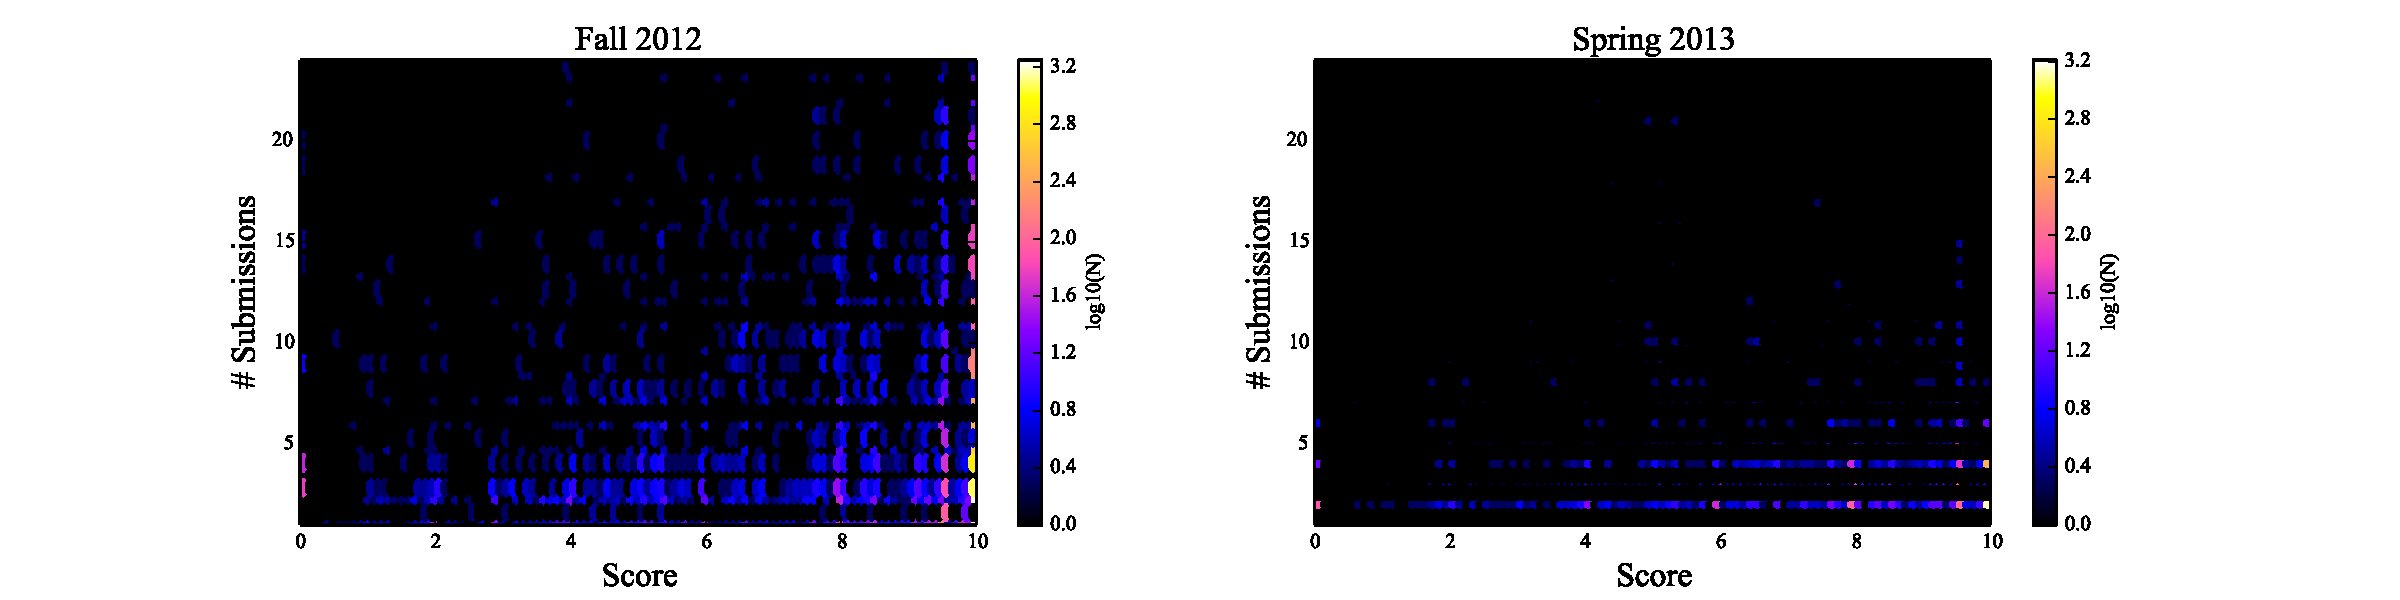
\includegraphics[width=\textwidth]{plots/score-2d-histogram-fall2012-spring2013.pdf}
  \vspace{-0.8cm}
  \caption{Heat maps correlating scores for the ``Huffman'' assignment and the number
  of required submissions.}
  \label{fig:2d-histogram}
\end{figure*}

\begin{figure}[ht!]
  \centering
  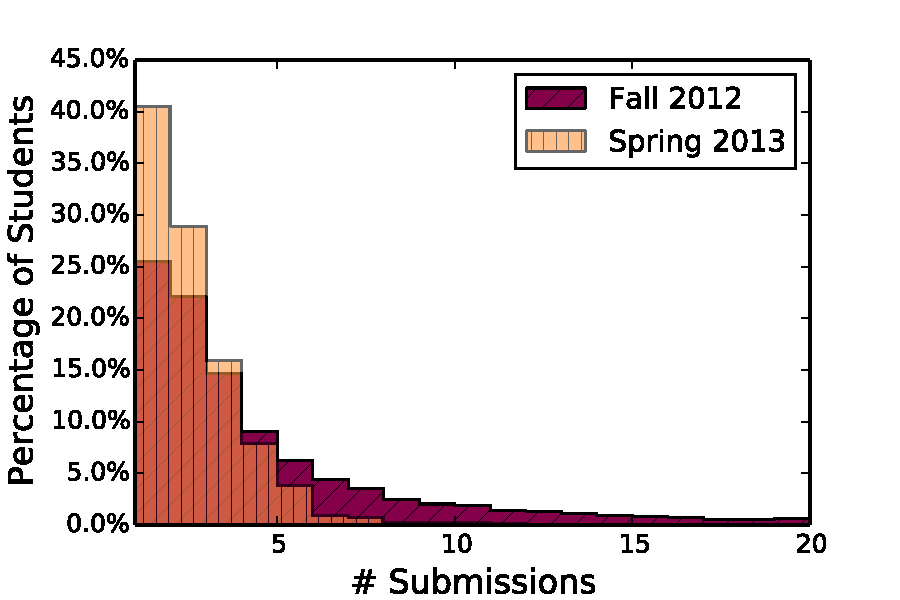
\includegraphics[width=\columnwidth]{plots/top-scores-submissions-histogram.pdf}
  \vspace{-0.7cm}
  \caption{The number of submissions required to achieve a perfect score in the ``Huffman'' assignment.}
  \label{fig:top-scores-submissions}
\end{figure}

All survey results have been released as part of the \textsc{progfun-stats} open-source
project~\cite{progfun-stats}. The survey data is available in simple
plain text formats, such  as tab-separated values. Thus, it is easy to process
and analyze the data in any general-purpose programming language. In addition
to the raw data set, \textsc{progfun-stats} provides a library extension for
the Scala programming language~\cite{Odersky-Spoon-Venners07} which makes it
easy to generate interactive, web-based visualizations\footnote{There is also a website showcasing more data and visualizations than shown in this paper, \url{http://lampwww.epfl.ch/~hmiller/progfun}}.

For example, Figure~\ref{fig:bar-chart} shows how to create a simple bar chart
that represents how ``worth it'' the course was for students, on a scale from
1 (disagree) to 5 (agree).

\section{Evaluation}
\label{sec:eval}

In this section, we analyze and evaluate a selection of the collected data.
First, we'll examine the role of the MOOC's tooling infrastructure
(e.g., IDEs, or the automated grader) in making distance learning more effective.
Next, we'll examine the background and motivation of MOOC participants which helps
explain whether MOOCs can be useful to professional software engineers. Finally,
as a third step, we evaluate the acceptance of our MOOC in a university setting.

\subsection{Tools for effective distance learning}

In this section we evaluate the use of two important tools: (a) the automated
grading system and (b) the Scala IDE for Eclipse plugin with the Worksheet IDE,
which was released specifically for use in the first iteration of the course.

\subsubsection{Automated grading system}

Before evaluating the grading system, we first clarify the respective grading
policies used. As mentioned in Section~\ref{sec:mooc-elements} the grading
policy changed between the Fall 2012 and the Spring 2013 iterations of the
course. In the Fall 2012 iteration, students could re-submit solutions as
often as they wanted without penalty until the submission deadline. In the
Spring 2013 iteration, students were allowed to re-submit only up to five
times; the sixth and later submissions would not give any credit. In both
iterations, the (valid) submission with the highest grade determined the final
grade for that assignment.

\paragraph{Usage of the submission system}

Figure~\ref{fig:2d-histogram} shows the correlation between the achieved
score for one particular assignment (an implementation of Huffman coding using
pattern matching) and the number of submissions required of each student to achieve that
score. For both the Fall 2012 and the Spring 2013 iterations of the course,
the largest concentration of students at or close to the perfect score
(10). In fact, both plots in Figure~\ref{fig:2d-histogram} show that
for a large number of students, only five submissions or less were required to
achieve their final/best score.

For the Fall 2012 plot, for example, each bright yellow dot
along the y-axis and concentrated around a score of 10 represents approximately 1,200-1,700
individual user submissions. Above 5 submissions however, the density of individual user submissions
drastically drops to approximately 250 or less individual user submissions.
This suggests that to achieve a higher score (even when submissions are unlimited),
a higher number of submissions was {\em not usually necessary}.

However, for the Fall 2012 iteration there are still thousands of students
with 10 or even 15 submissions. The results for the Spring 2013 iteration are
quite different: most people achieved their final score after only two or four
submissions. This difference stems from the adoption of a different grading policy used in
the second iteration of the course: no credit for
the sixth and later submissions. This is clearly reflected in the changed
submission statistics.

\begin{figure}[ht!]
  \centering
  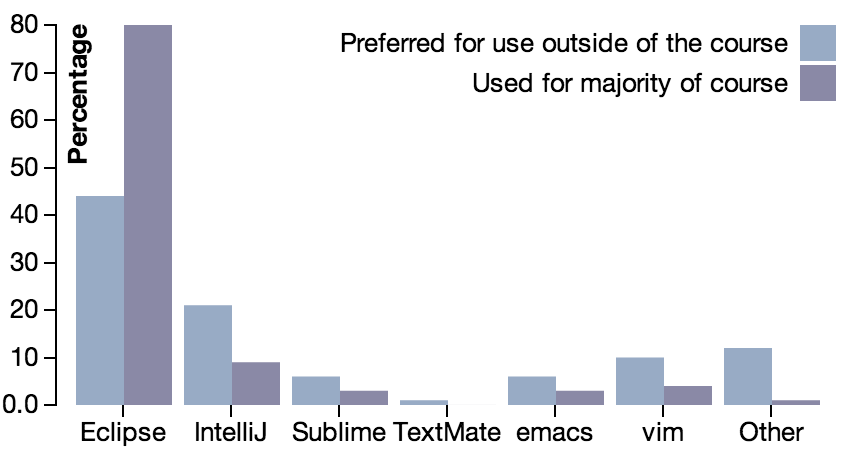
\includegraphics[width=\columnwidth]{plots/ides.png}
  \caption{Results for the survey questions, what is your preferred editor, for use outside of this course?, and what editor did you end up using for the majority of the course?}
  \label{fig:ides}
\end{figure}


However, interestingly, there are still a significant
number of students who also submitted six or more times (thus earning no additional
credit); this is a clear indication that the automated grading and feedback
was also used for learning without improving one's score.

This change in the grading policy had an interesting effect on the quality of
initial submissions. Figure~\ref{fig:top-scores-submissions} shows the change
in the number of submissions of students who achieved a perfect score on a
particular assignment. The change in submission behavior between the Fall 2012
and Spring 2013 offerings is quite noticeable.
In the Fall 2012 iteration about 25\% of those perfect-scorers needed only one
submission, whereas in the Spring 2013 iteration this percentage grew to about
40\%. For perfect-scorers who needed two submissions, the difference between
the two iterations is not as large, but still significant (an increase of
about 30\%).

\begin{figure*}[htb!]
  \centering
  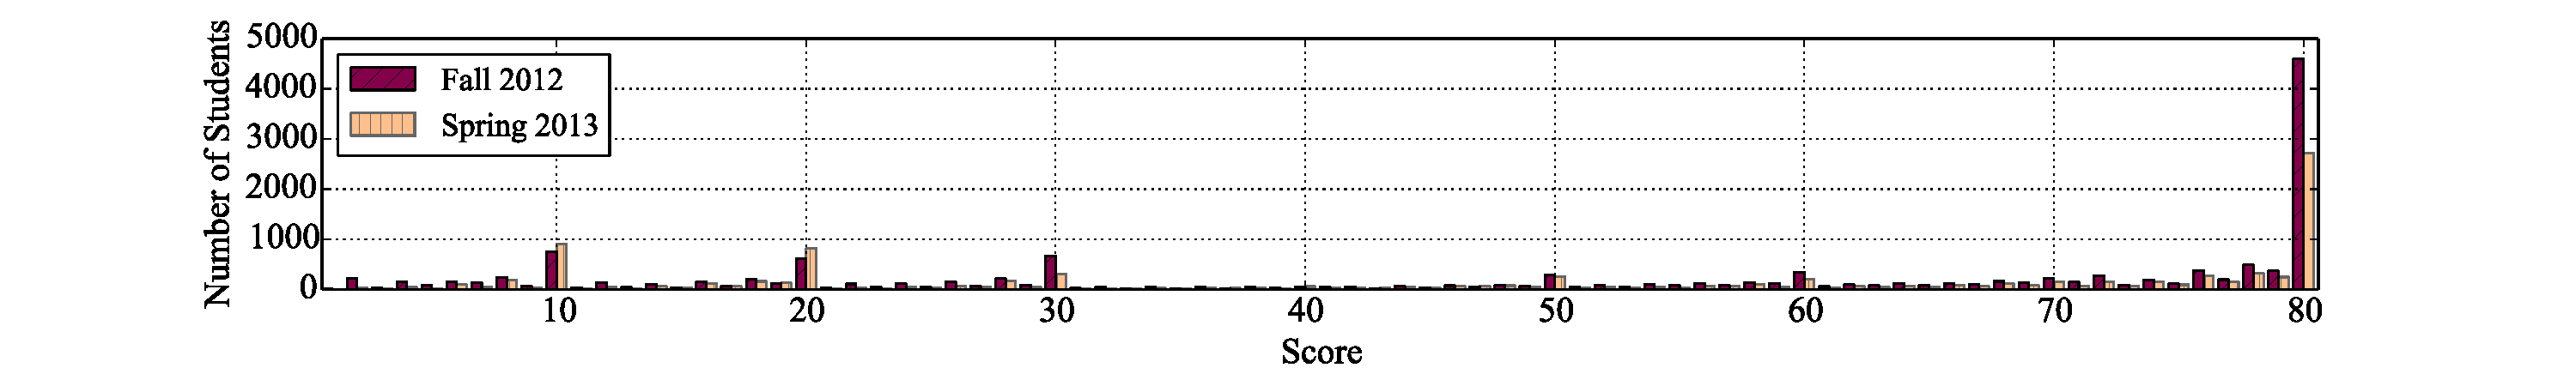
\includegraphics[width=\textwidth]{plots/final-scores.pdf}
  \vspace{-0.8cm}
  \caption{Final scores after the entire course (both iterations).}
  \label{fig:final-scores}
\end{figure*}

\begin{figure}[ht!]
  \centering
  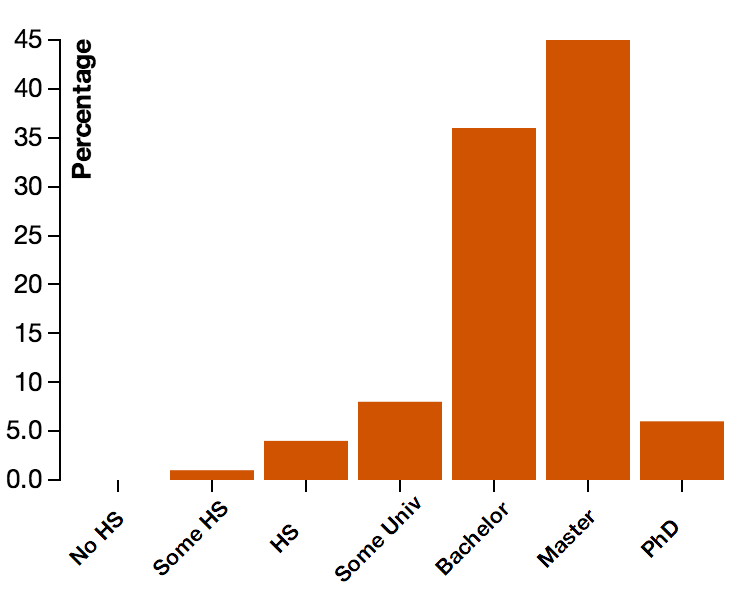
\includegraphics[width=0.85\columnwidth]{plots/education.png}
  \vspace{-0.5cm}
  \caption{Educational background of MOOC participants}
  \label{fig:education}
\end{figure}


% \paragraph{Summary}

% The interaction with the submission system worked well, since (1) people used
% it beyond just getting assignment scores (shown in heat map for 2013 in Figure~\ref{fig:2d-histogram}), and (2)
% the heat map shows people improved scores by submitting again and again.


\subsubsection{The Worksheet IDE plugin}

Figure~\ref{fig:ides} shows survey respondents' code editor preferences both
(a) preferred for use outside of the course, as well as (b) the code editor used
for a majority of the course. The results show that
80\% of all students prefer to use the Scala IDE for Eclipse for the course.
For almost half of those students, Eclipse is not their preferred IDE for projects outside
the course. One feature that was only available in the Scala IDE for Eclipse
during the first course iteration is the Scala worksheet, introduced in Section
\ref{sec:tooling-automated-grading}. The students are encouraged to use the
worksheet for testing their code, and the feature is also used by the lecturer
in the videos. There are other reasons that explain the popularity of the
Scala IDE: it is straightforward to download and install, the assignments can
be easily imported into the IDE, and it is the recommended code editor for the
course.

\subsection{Not just for students}

In this section, we evaluate the background and motivation of MOOC participants,
in an effort to show that MOOCs can be useful to professional software engineers.

Figure~\ref{fig:education} shows a summary of the educational background of
participants of the MOOC. Surprisingly, nearly half of all respondents has completed a
Master's degree. Thus, the question arises: how relevant are the topics of the
MOOC to participants' professional work? Survey results indicate that about
40\% of respondents plan to apply the learned knowledge at work (see
Figure~\ref{fig:where-apply}). Thus, participants' professional work appears
to be a strong motivating factor. We suspect that the fact that the Scala
programming language is not yet taught in many universities could also
contribute to the popularity of the MOOC to (recent) university graduates.

\begin{figure}[ht!]
  \centering
  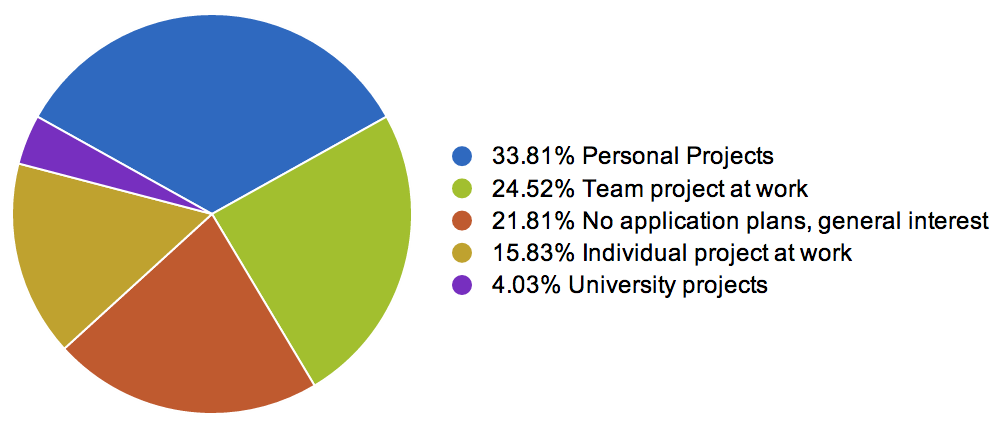
\includegraphics[width=\columnwidth]{plots/where-apply.png}
  \caption{Results for the survey question: where do you plan to apply what you've learned in this course?}
  \label{fig:where-apply}
\end{figure}

Interestingly, professional participants felt like the course was well worth
their time even more so than across all participants. Figure~\ref{fig:worth-it-apply-it}
shows the results of the question, ``do you feel the course was worth the time you invested in it?"
for two groups of individuals; ``all respondents" as well as those respondents who
indicated they were interested applying knowledge gained from the course towards a
(group or individual) project at work. For the Fall 2012 offering, for example, the
results show that 71\% of professionals (i.e., 2,148/3,203 professional respondents)
felt the course was well worth their time, as opposed to 68\% (5,077/7,492) for all respondents.
Thus, progfun was quite ``effective'' for practicing software engineers, indicating
that some MOOCs can be an effective training tool for professional software engineers.

Another interesting observation that can be garnered from Figure~\ref{fig:worth-it-apply-it}
is that the difference in how ``worth it" progfun was to professionals vs all respondents
is large enough to be statistically significant, but still not disparate enough to indicate
that potential newcomers (potentially 57\%, or some 4,289/7,492 respondents) struggled or were
hindered by the Scala tooling and build infrastructure. On the contrary, newcomers and
Scala professionals alike followed suit in their positive overall experience with the course.

% still left
% the course with a positive
% From Figure~\ref{fig:worth-it-apply-it}, it's evident that there is not a large disparity in how ``worth it'' the course was for complete newcomers to Scala and its ecosystem as well as people familiar with the Scala tool-chain (those who work with Scala on a daily basis). That is to say that the Scala tool-chain and ecosystem weren't a hindrance.

Furthermore, a certificate of completion was issued. Unlike languages
established in industry for many years, there is no standard Scala
certification for developers; the completion certificate could be regarded by
many as the closest substitute.


\begin{figure*}[ht!]
  \centering
  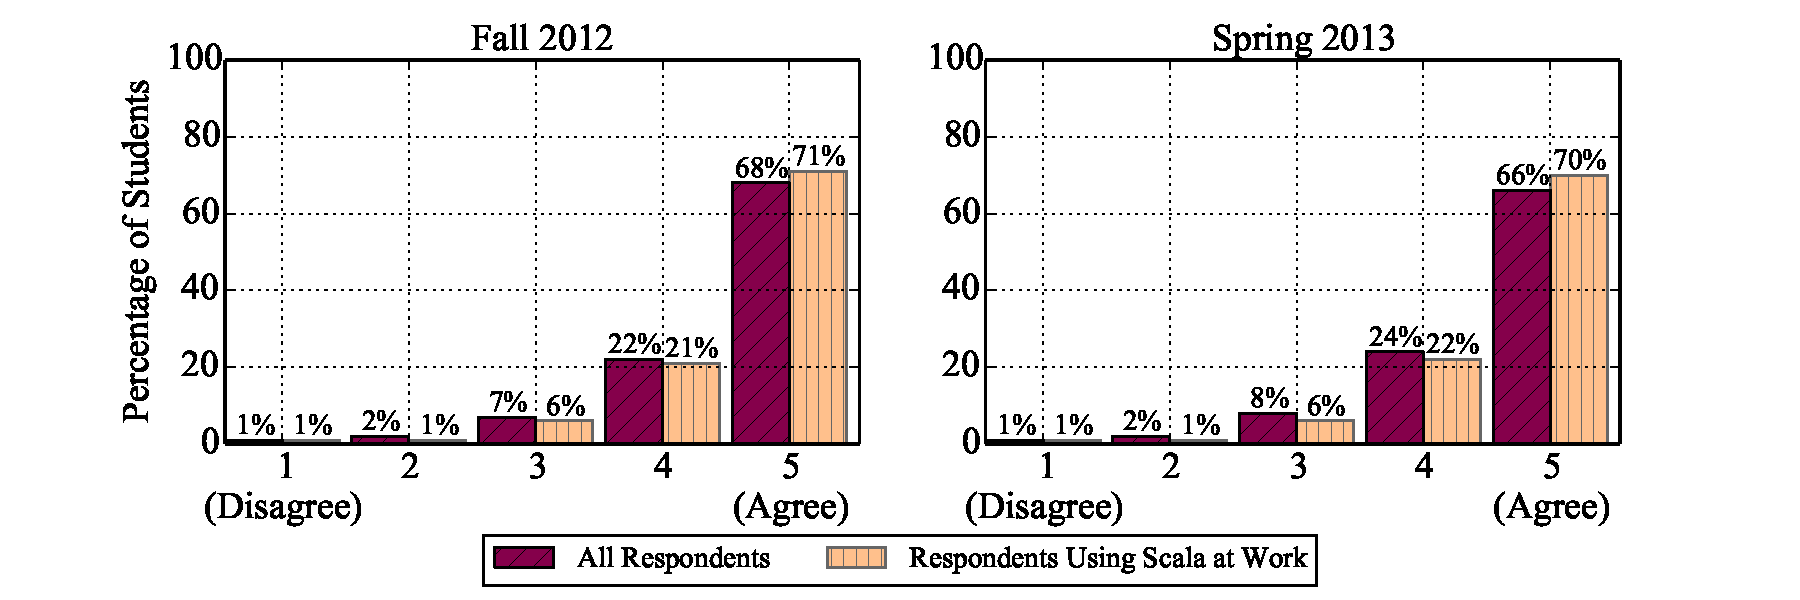
\includegraphics[width=\textwidth]{plots/worth-it-apply-it.pdf}
  \caption{Correlated results from two groups of individuals for the survey question: do you feel the course was worth the time you invested in it? Shown are ``all respondents'', and respondents that indicated they were interested applying knowledge gained from the course towards a (group or individual) project at work.}
  \label{fig:worth-it-apply-it}
\end{figure*}

\begin{figure*}[ht!]
  \centering
  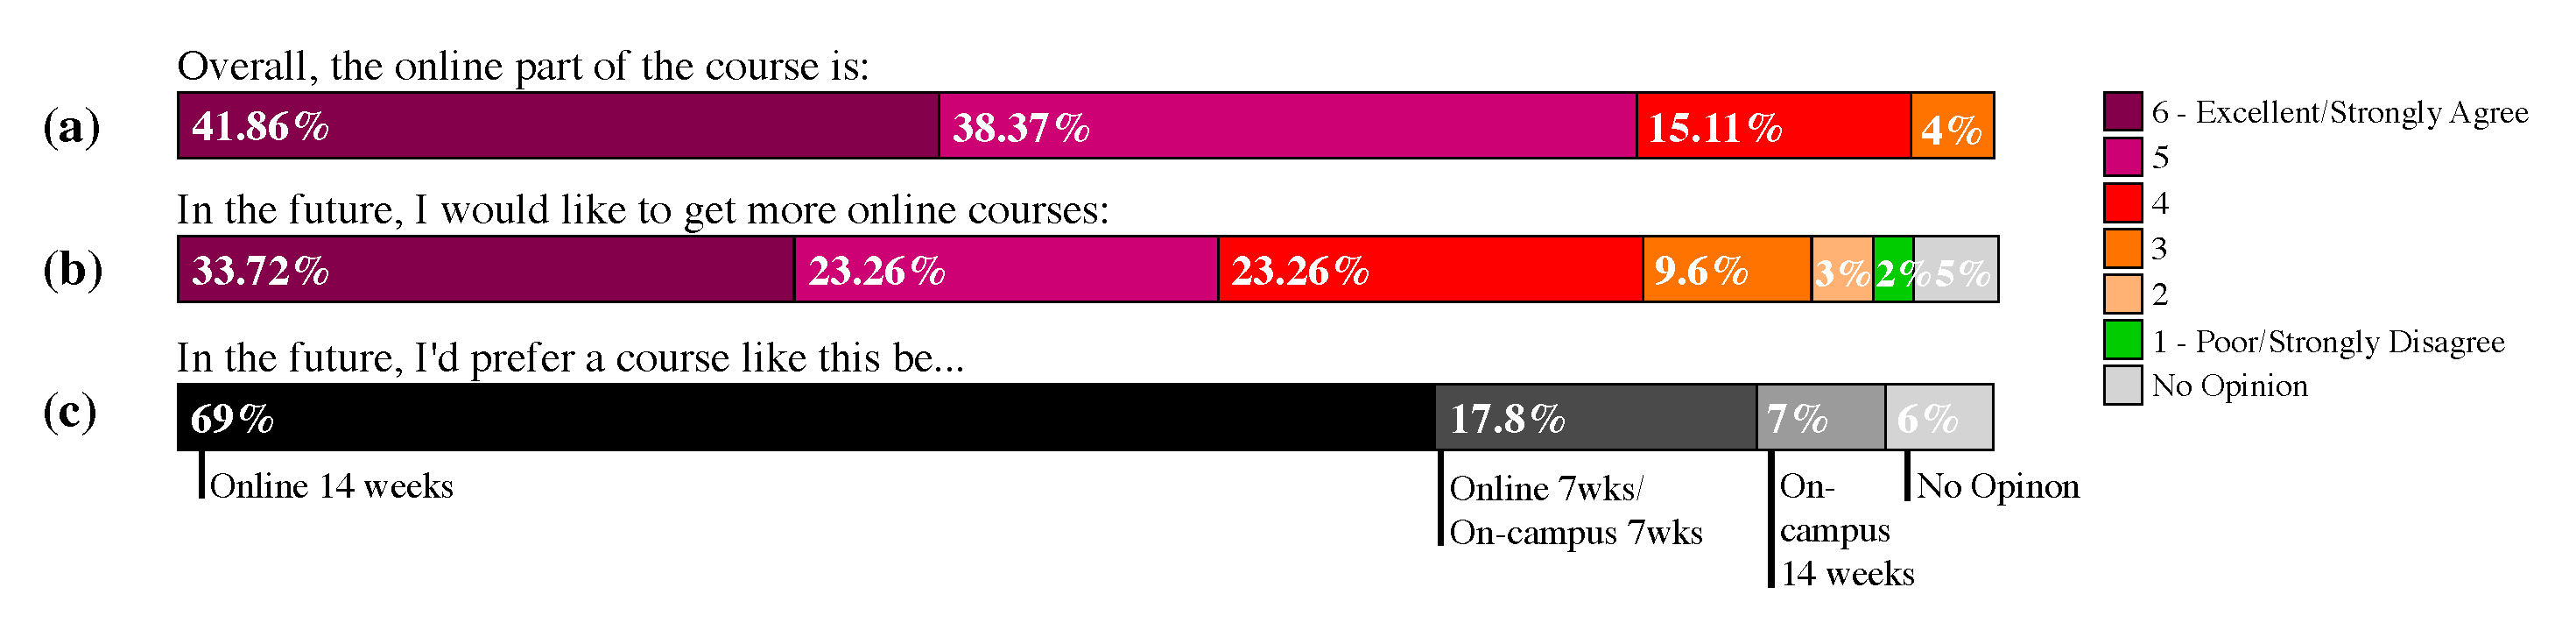
\includegraphics[width=\textwidth]{plots/epfl-course-eval.pdf}
  \caption{MOOC-related responses from EPFL's specialized course evaluation, given to on-campus EPFL students following the conclusion of the online MOOC half of the course, as well as the offline traditional half of the course.}
  \label{fig:epfl-course-eval}
\end{figure*}

\subsection{Acceptance and student evaluation}

Figure~\ref{fig:epfl-course-eval} shows the result of our survey among
students at EPFL who took both the MOOC as well as the subsequent second part
of a regular on-campus course.

The results show that the online part was very
well received: in Figure~\ref{fig:epfl-course-eval}(a) about 80\% of all respondents
think the online part was very good or excellent.
In Figure~\ref{fig:epfl-course-eval}(b), about 57\% of respondents agree or strongly
agree that they would like to have the opportunity to take more online courses.

In fact, 69\% of students say they would prefer to
have all 14 weeks of {\em a semester-long course like principles of functional programming}
be online; only about 18\% think that the configuration which was actually used,
namely 7 weeks online, 7 weeks on-campus, was ideal. The results shown in
Figure~\ref{fig:epfl-course-eval}(e) show that EPFL students fully accepted the novel
online part, and in fact preferred it compared to the traditional on-campus part.

Figure~\ref{fig:epfl-course-eval}(c-d) also show that students seem to prefer the online
help forums over EPFL's traditional on-campus help during weekly exercise sessions, with
nearly 50\% of all students rating the online forums as excellent or very good, as opposed
to a mere 30\% of students rating the traditional in-person exercise sessions as excellent
or very good.
% While this
% might have been evident in the lower attendance numbers for the weekly exercise sessions as
% compared to previous years,

\section{Related Work}
\label{sec:related-work}

The well-known MOOC on software engineering organized by Fox and
Patterson~\cite{FoxP12} has had around 50,000 registered students in its first
iteration, and is thus comparable in size to our course; however, no survey of
a comparable size was conducted among participants of the MOOC. Moreover, our
selection of questions provides new insights, related to the interplay of
MOOCs with professional software engineering, in particular.

Vihavainen et al. report on a MOOC (``Helsinki MOOC") on introductory computer
science with an emphasis on programming~\cite{VihavainenLK12}. Compared to the
Helsinki MOOC, our course had a number of registered students two orders of
magnitude larger. Moreover, the Helsinki MOOC targets introductory
programming, whereas our course targets advanced programming principles. As a
result, our course was very popular especially among advanced developers who
already have a Bachelor's or Master's degree. The Helsinki MOOC does not treat
university students and MOOC participants equal with respect to the material
used for exercises: the students in their university course are beta testers
of the exercise material; thus, only after this beta test and necessary
adjustments is the material released to non-local MOOC participants. Other
organizational differences exist. For example, they give formal credits for
``apprentices'' who are unpaid ``advisors'' among fellow students with limited
responsibilities. Their Extreme Apprenticeship (XA) learning methodology
required a staff of around 20 persons associated with the course, with
different roles and responsibilities. It is unclear whether the XA methodology
would scale to a course of the scale of progfun (50,000 registered students
versus 500 registered students).

Looking back into the literature a bit further, there also exists a body of
of work on automated grading of programming, beginning as early as the late 1960's,
much of which is nicely summarized in a survey by Douce et al.~\cite{Douce}. These approaches
are somewhat similar in that they are predominantly test-based. That is, even the very
first automated testing systems introduced by Hext et al.~\cite{Hext69} sought to compare
some stored testing data with data from a running application. Some of these early systems,
such as Assyst~\cite{Assyst}, even developed methodologies for testing for qualities such as
efficiency and modularity, though naturally, none of these systems are able to be run
concurrently in the cloud. Similar, however, is RoboProf~\cite{RoboProf}, a web-based system for
testing code submissions and providing feedback, though not suited to scale as necessary for use with MOOCs.
Meanwhile, more recent work~\cite{PLDI13} differs in that its focus is not test-based, but
rather, based on program synthesis – it's additionally not suited to our use-case because it
provides too much assistance.

\section{Conclusion}
\label{sec:conclusion}

%
% The following two commands are all you need in the
% initial runs of your .tex file to
% produce the bibliography for the citations in your paper.
\bibliographystyle{abbrv}
\bibliography{sigproc}  % sigproc.bib is the name of the Bibliography in this case
% You must have a proper ".bib" file
%  and remember to run:
% latex bibtex latex latex
% to resolve all references
%
% ACM needs 'a single self-contained file'!
%
%APPENDICES are optional
%\balancecolumns
\end{document}
